\documentclass{VUMIFInfKursinis}
%\usepackage{algorithmicx}
%\usepackage{algorithm}
%\usepackage{algpseudocode}
%\usepackage{amsfonts}
%\usepackage{amsmath} don't need becouse mathtools already inports
\usepackage{mathtools}
%\usepackage{bm}
\usepackage{color}
\usepackage{hyperref}  % Nuorodų aktyvavimas
%\usepackage{url}


%My personal additions
\graphicspath{{img/}}
\newif\iffast{} %degaults to false
\fasttrue{}
\iffast{}

	\usepackage[rgb,dvipsnames]{xcolor}
	\usepackage[colorinlistoftodos,prependcaption,textsize=footnotesize]{todonotes} 

	\addtolength{\oddsidemargin}{3cm}
	\addtolength{\evensidemargin}{3cm}
	\addtolength{\textwidth}{-3cm}

	\reversemarginpar{}
	\setlength{\marginparwidth}{5.5cm} 
\else
\fi
%\usepackage{booktabs}

% Titulinio aprašas
\university{Vilniaus universitetas}
\faculty{Matematikos ir informatikos fakultetas}
\department{Informatikos katedra}
\papertype{Kursinis darbas}
\title{Dokomentų klasterizacija}
\titleineng{Document clustering}
\status{4 kurso 1 grupės studentas}
\author{Dominykas Ablingis}
% \secondauthor{Vardonis Pavardonis}   % Pridėti antrą autorių
\supervisor{lekt. Rimantas Kybartas}
\date{Vilnius \\ \the\year}

% Nustatymai
\setmainfont{Palemonas}   % Pakeisti teksto šriftą į Palemonas (turi būti įdiegtas sistemoje)
\bibliography{bibliografija} 

\begin{document}

\iffast{}
	\newcommand{\rewrite}[1]{\todo[linecolor=red,backgroundcolor=red!25,bordercolor=red]{#1}}
	\newcommand{\needsource}[1]{\todo[linecolor=blue,backgroundcolor=blue!25,bordercolor=blue,]{#1}}
	\newcommand{\toadd}[1]{\todo[linecolor=OliveGreen,backgroundcolor=OliveGreen!25,bordercolor=OliveGreen,]{#1}}
	\newcommand{\note}[1]{\todo[linecolor=Plum,backgroundcolor=Plum!25,bordercolor=Plum]{#1}}
	\newcommand{\thiswillnotshow}[1]{\todo[disable]{#1}}
	\listoftodos[Notes]
\else
	\newcommand{\rewrite}[1]{}
	\newcommand{\needsource}[1]{}
	\newcommand{\toadd}[1]{}
	\newcommand{\note}[1]{}
	\newcommand{\thiswillnotshow}[1]{}
\fi

\maketitle
\tableofcontents

%My macros

\newcommand{\ltang}[2]{#1 (angl.\  \textit{#2}) }
\newcommand{\BigO}[1]{$\mathcal{O}(#1)$}

\sectionnonum{Sąvokų apibrėžimai}
%Sutartinių ženklų, simbolių, vienetų ir terminų sutrumpinimų sąrašas (jeigu ženklų, simbolių, vienetų ir terminų bendras skaičius didesnis nei 10 ir kiekvienas iš jų tekste kartojasi daugiau nei 3 kartus).
\begin{itemize}
	\item cluster
	\item clustering
	\item document
	\item corpus
	\item term – termas dar vadinamas (tokens, words,terms or attributes)
	\item token
	\item feature
	\item online
	\item ofline
	\item supervised
	\item unsupervised
	\item \ltang{matmenų redukcija}{dimensionality reduction}
\end{itemize}

\sectionnonum{Įvadas}
%Įvade apibūdinamas darbo tikslas, temos aktualumas ir siekiami rezultatai. Darbo įvadas neturi būti dėstymo santrauka. Įvado apimtis 1–2 puslapiai.
Šiais laikais kai kiekvienas žmogus turintis priėjimą prie interneto gali dalintis informacija, daugybė knygu yra skaitmenizuojamos kiekvieną dieną ir mokslo institucijos dalinasi savo moksline informacija, pasiekemos informacijos kiekis didėja su kiekviena diena ir pagrindinė problema nebėra informacijos trūkumas, o atradimas ko reikia. Tam spresti buvo ir yra kuriama ivairūs mechanizmai: paiškos varikliai\ldots Šiame darbe autorius nagrinės viena iš šios problemos sprendimo metodų, klasterizacijos algoritmus ir jų panaudojimą textinems dokumentams. %Klasterizacijos algoritmai priklauso neprižiūrimo mokymosi \textbf{tipui} ir pagrinde naudojami.

Šiandieninėje visuomenėje prieinamos informacijos kiekis didėja su kiekviena diena ir pagrindinė problema yra ne informacijos trūkumas, o jos gausa ir galimybė surasti reikiamą informaciją. Paieškos programos gali pateikti didelius kiekius tekstinių dokumentų, bet reikiamo dokumento paieška užima daug laiko ir be to, ne visada gauta informacija atitinka paiešką. Tekstinių dokumentų paieškos procesui palengvinti ir pagreitinti gali būti taikomi klasterizavimo metodai, kurie yra pakankamai gerai žinomi ir jau seniai naudojami duomenų klasterizavimui.  Klasterizavimo metu  dokumentai pagal savo turinį suskirstomi į klasterius vadovaujantis tam tikrais kriterijais, pvz., pagal temą, pagal dokumento naujumą ir pan. 



\section{Pagrindinė tiriamoji dalis}
%Pagrindinėje tiriamojoje dalyje aptariama ir pagrindžiama tyrimo metodika; pagal atitinkamas darbo dalis, nuosekliai, panaudojant lyginamosios analizės, klasifikacijos, sisteminimo metodus bei apibendrinimus, dėstoma sukaupta ir išanalizuota medžiaga.
\toadd{Reikia nuspresti ką konkrečiau tirsiu ir tai aprašyti.}
Darbo tikslas – mokslinės literatūros apie dokumentų apdorojimą ir klasterizavimą apžvalga ir analizė  

Darbo uždaviniai: 
\begin{enumerate}
	\item Panaudojimo sritys
	\item Dokumentų klasterizavimui naudojamų įrankių ir metodų apžvalga.
	\item Dokumentų klasterizavimo proceso žingsnių aprašymas
	\item Kylantys iššūkiai  
	\item Susijusios problemos 
\end{enumerate}

Kursiniame darbe buvo siekta susipažinti su moksline literatūra, išanalizuoti egzistuojančius dokumentų klasterizavimo metodus ir įrankius, kurie bus išbandyti taikomojo pobūdžio  kursiniame darbe apie lietuviškų dokumentų klasterizavimą.

Šiame darbe taip pat bus paminėtos kitos su dokumentu klasterizacija susijusios problemos ir ši informacija bus išdėstyta eilės tvarka kaip būtu sprendžiamos užduotys.
\begin{enumerate}
	\item Duomenų išgavimas iš skirtingų tekstinių dokumentų formatų
	\item Duomenų apdorojimas
	\item Algoritmai
	\item Algoritmų testavimas
	\item Rezultatų vizuoalizacija
\end{enumerate}


\section{Dokumentu klasterizavimo pritaikymai}
Dokumentu klasterizacija turi daug pritaikymų ivairiose verso ir mokslo srityse. Iš pradžių, dokumentų klasterizacija buvo tiriamas \ltang{informacijos išgavimo sistemomų}{information retrieval systems} tikslumui ir kokybei pagerinti. Toliau išvardinsim keletą pagrindinių klasterizavimo panaudojimo sričių\cite{jajoo2008document}.
\begin{itemize}
	\item \textbf{Ieškant panašių dokumentų} Ši funkcija dažniausiai panaudojama kai vartotojas perskaito patikusi straipsni ar tarp paieškos rezultatų randa „patikusi“ dokumentą ir nori daugiau panašių straipsnių ar rezultatų. Šis atvėjis vertingas nes klasterizacija sugebėjo surasti dokumentus kurie yra konceptuoliai panašūs vietoj paieška paremtų metodų kurie gali atrasti tik ar dokumentas turi panašių žodžių su paieškos užklausa.  
	\item \textbf{Didelių dokumentų rinkinių orangizavimas} Dokumentų paieška paskirtis yra surasti dokumentus kurie yra aktualūs pagal pateiktą užklausą, bet tai nėra tinkamas būdas susidaryti bendram vaizda iš viso nekategorizuotų dokumentų rinkinio. Šios problemos išukis yra suorganizuoti dokumentu į grupes (taksonomija) idnetiškas tokioms kurias sukurtu žmogus turint pakankamai laiko. Tada šį grupavimą panaudoti kaip naršymo sąsają lengvesniam dokumentų naršymui. 
	\item \textbf{Besiduplikuojančio turinio aptikimas} Daugybėja sričių yra atvejų kai reikia rasti duplikatus ar beveik duplikatus. Nors trivialiems atvėjams pakanka primityvių metodų, bet sudetingesniems atvejams klaserizacija yra vienas iš sprendimų. Klasterizacija yra aktyviai naudojama plagyjavimo detekcijai, straipsnių apie tą pati įvyki iš skirtingų publikacijų suradimui, paieškos rezultatų pertvarkymui (norint didesnės diversijos tarp pirmų rezultatų).
	\item \textbf{Rekomendacijų sistemos} Šioje problemoje vartotojui yra rekomenduojami straipsniai rementis vartotojo jau perskaitytais straipsniais (perskaitytų straipsnių istorija). Ši problema dažniausiai sprendžiama lyginant vieno vartotojo skaitymo istorija su kitų vartotojų, deja šis sprendimas dažniausiai rekomenduoja pagal populiarumą straipsnius \rewrite{rekomentuoja dokumentus kurie yra populirarus ir netolygiai paskirsto rekomendacija \ldots} Tuo tarpu, lygintat perskaitytus straipsnius su jau sudarytais klasteriais tikėtinai gaunamos obijektyvesnės rekomendacijos. Taip pat galima panaudoti vartotojų perskaitytu straipsnių sarašus pagerinant klasterių kokybei.\footnote{Tai jau būtu prižiūrimo mokymo problema}.
	\item \textbf{Paieškos variklių optimizacija} Klasterizacija labai vertinga paieškos rezultatų kokybę ir spartą. Tai atliekama pirma lyginant užklausą su klasteriais vietoj to, kad lyginti su kiekvienu dokumentu atskirai. Tuopačiu tai palengvina rezultatų rikiavimą, nes dalis klasterizacijos metodų leidžia lyginti konkretų dokumentą su visu klasteriu.  
\end{itemize}

\section{Duomenų išgavimas, apdorojimas ir pavertimas į patogia formą}
	Jeigu dirbame su iš anksto neparuoštu \ltang{duomenų rinkiniu}{data set}, reika pradėti nuo duomenų apdorojimo\cite{kadhim2014text}. Šiuo atveju duomenys yra dokumentai kurie gali būti pateikti įvairiais formatais: moksliniai darbai Latex formatu, internetiniai puslapiai html fotmatu, elektroninės kngyos \ldots Šiuos dokumentus reikia transliuoti į patogesnią analizei formą. Taip pat dažnai susiduriant su žmogišku tekstu reikia ji paildomai apdoroti. Dažnai išemami stop words (nekaitomos kalbos dalys) (nebent atilekama frazių analizė) ir ženklai (!?\ldots), žodžiai pakeičiami į bendrinię formą, kad supaprastini apdorojamą teksta neprarandant gilesnės teksto minties. 

\subsection{Duomenų išgavimas}
\needsource{cite specifications and add more details about scraping}
Informacijos išgavimas iš interneto ir kitų šaltinių

\subsubsection{XML/HTML dokumentai}
XML atvėju \texttt{<tag>Content</tag>} tag galime interpretuoti kaip kintamajį. Galima interpretuoti kaip  kintamoji Content kaip kintamojo reikšmę, arba tag kaip teksto anotacija. Bet tai negalioja html atveju tagai Skirti nurodyti svetainės išdėstymą. Pavyzdžiui <h1> dažniausiai reiškia pavadinimą ar antrašnę ir XML atvėju turbūt būtu <title>. Taip pat Interneto svetainės turi  kitos tekstinės informacijos kaip navigacija, komentarai, kontaktai ir panašiai. Šia problema sprendžiam keliais žingsniais:
Pirma galime pasinaudoti tuo kad HTML yra DOM … todėl tai yra medžio struktūra. Supaprastinti darba galima apdorojant tik specifines šakas, bet tarp skirtingu svetainių šis medis atrodys skirtingai, taigi to pakaks tik dalinai
Kurkas paprastesnis būdas pasinaudoti statisniu metodu (Finn’s method). Atskireme tagus į skirtus tekstui (<bold>, <italic>\ldots) ir neskirtus (<head>, <body>\ldots). Tada stebime tagų (neskirtu tekstui) pasiskirstyma puslapyje lyginat su tekstu, ten kur ju daug galime numanyti kad tai nera pagrindinis puslapio turinys ir vice versa. Tai pavaizdavus grafike pamatytume išsilyginima

\subsubsection{PDF}
\ltang{PDF}{Portable Document Format} Dokumentų formatas skirtas lengvam dokumentų dalinimuisi tarp skirtingų sistemų. PDF yra kurkas sudėtingesnis formatas ir dėl to duomenų išgavimas tampa painesnis. PDF dokumentai išdėstymui ir grafikai naudoja PostScript formatavimo kalbą, taip pat savyje išsaugo reikalingus šriftus ir turi struktūrinę sistemą kuri išsaukgo visus šiuos duomenis į vieną failą ir kur tinkama panaudoja duomenų suspaudimą.\toadd{Detalesnis aprasymas ir budai išgauti tekstą}
Dažnai internete galime sutikti knygų variantus kurie buvo tiesiai nuskenuoti ir idėti pdf dokumentą kaip paveikslėliai. Norint iš tokio dokumento išgauti tekstą reiktų panaudoti {Teksto atpažinimas}{OCR (optical character recognition)}

\subsubsection{Tex}
Tex yra dokumentų maketavimo kalba ypač dažnai naudojama matematikos, fizikos ir kommpiuterių mokslo srityse. Dali moksliniu darbų ir knygų galima prieti netik PDF bet ir autorių rašta Latex versija.

\subsubsection{Elektroninių knygų formatai}
\begin{itemize}
	\item ePub
		XML pagrindu paremtas, atviras formatas
	\item MOBI

	\item AZW3
		Formatas paremtas daline HTML5 ir CSS3 funkcijų implentacija. 
\end{itemize}

\subsection{Teksto apdorojimas}
\ltang{Teksto apdorojimas}{Text preprocessing} tekstą iš patogios žmogui formos paverčia į patogia kompiuteriui. Šiame poskyryje pateikti žingsniai išdėstyti populiariai naudojama eilės tvarka, bet visda reikia atkreipti dėmesi koks tyrimas atliekamas ir pagal tai spresti ar žingsniai yra reikalingi ir ar jiems nereikia modifikacijų (Pvz. Stemming žingsnyje iš „geras“ ir „negeras“ taptu tuo pačiu žodžiu kas būtu netinkama \ltang{emocijų nustatymui}{Emotion Detection}). Šie žingsniai netik padeda pagerinti našumą, bet ir rezultatų kokybę\cite{mugunthadevi2011survey}.

\subsubsection{Tokenization – teksto išskaldymas į reikšmingas dalis}
Tai dažniausiai būna primas teksto apdorojimo žingsnis, jo metu iš neapdoroto teksto išgaunami atskiri tokenai (Žodžius, frazes atributai \note{rask tinkama reikšmę}) ir patalpinama į patogia duomenų struktūra tolesniam apdorojimui (Šiame žinksnyje taip pat panaikinami visi skyrybos ženklai ir nespausdinami simboliai) \note{ar TAB, ENTER, \@, \# ir kiti simboliai irgi yra skyrybos ženklai}. Dažniausiai naudojama \ltang{žodžių maišelio}{bag of words} duomenų struktūra (nors ji praranda teksto eiliškumą) \note{Detaliau aprašyk BOW}. Vėliau šie žodžiai bus naudojami kaip ideksai žodyne.
Tekstų tokenizacija yra vis dar aktyviai tiriama sritis, ypač kalboms kuriose nėra aiškių žodžių ribų \note{parodyti pavizdžių apie Scriptio continua}. Taip pat problematiški žodžiai su ženkalais viduje: I.B.M.\; pre-diabetes. Tokiais atvėjais netinka nei atskirti nei sujungti nes abejais atvėjais prarandama prasmė ir sukuremi netikslūs token’ai. Yra keli sprendimai: vienas padaryti abu (dalinti ir jungti) tokiu butu atsiranda daugiau triukšmo duomenyse, bet tai neturetu buti problema jeigu tvarkingi sureguliuoti svoriai. 
Morfologinė variacija. Problema su žodžiais kur viena šaknis gali turėti kelias skirtingas prasmes. Arabų kalba ypač sudėtinga šituo atžvilgiu nes turi palygint mažai šaknų, bet labai daug variacijų. Pokyčiai gali būti prieš, po ir pačioje šaknyje.

\subsubsection{Nereikšmingų žodžių pašalinimas}
\ltang{Nereikšmingi žodžiai}{stop-words} – tai tokie žodžiai (įvardžiai, prielinksniai, jungtukai ir pan.) kurie jungia reikšmingas teksto dalis, bet patys nesutekiai tekstui reikšmės. Šiame žingsnyje taip pat gali būti pašalinti skaičiai ir specifiniai simboliai. Reikia atkreipti dėmėsį, kad skirtingos sritys gali turėti skirtingus stop-word (pvz internete žodis “click” dažnai naudojamas ir nėra labai prasmingas). Taip pat kai kurios frazės gali būti sudarytos iš stop-word ir turėti prasmę (“to be or not to be”).\toadd{Search for Lithuanian equivalent}.\\
Šiai spresti įprastai sudaromas arba naudojamas specifinės kalbos ir srities žodynų junginys. Jeigu nėra galimybės gauti jau sudaryto žodyno, taip pat galima jį sugeneruoti iš turimų žodžių. Jeigu išgautus žodžius išrikiuotume pagal jų dažnį, galime atmesti dažniausius (nes galime spresti, kad jie nereikšmingi ir nepadės atskirti vieno teksto nuo kito) ir rečiausius (nes jie taip pat bus nereikšmingi, nes nesies skirtingų dokumentų). Generuojant savą žodyną gali prireikti šį ir sekany žingsni sujungti. 

\subsubsection{Stemming – žodžio šaknies išgavimas.}
Dažnai programos (angliškai vadinamos stemmers) gauna žodį ir gražina jo šaknį. Egzistuoja keli implementacijos būdai: \\
Naudojant parengtas taisykles ir išimčių žodynus. Jeigu esamai kalbai ar sričiai nėra žodyno, tada implementavimui reikia kalbos eksperto kurio pagalba būtu suprogramuojamos visos taisyklės ir išimtys. Šis metodas veikia gerai bet reikalauja daug laiko, yra sudetingas ir sunkiai apibendrinamas.
\\Kitas būdas panaudoti Stemminimo algoritmus, bet kaip ir su žodynais mažiau populiariom kalbom algortimai gali nebūti tinkamo algoritmo. \note{Nurodyti cituotus pavyzdžius ir galbūt jų veikimą}
\\Taip pat galima panaudoti raidžių n-gramos, panašiuose žodžiuose panašios n-gramos. Standartiškai Europinėms kalboms $n = 4$. Stemming’as gali ivykti skirtinguose apdorojimo etapuose priklausomai nuo užduoties.

\subsubsection{Sinonimiškumas ir Polisemija}
%TODO maybe merge with stemming 
Indexų pavyzdžiai: Wordnet, MeSH, taip pat yra daug statistinių metodų. Kartais prašoma vartotojų nurodyti kurią iš sinonimo reikšmių jie turėjo omeny arba vertinti paieškos rezultatus nurodant kurie atitinka o kurie ne, tokiu butu paieškos problema paversti į supervised learning problemą (relevance feedback).

\subsection{Dokumento reprezentacija}
Nors yra daugybė duomenų reprezentacijos/ (feature extraction) technikų, bet jeigu imanoma, geriausia naudoti tas kurios pritaikytos duomenų tipui\cite{alelyani2013feature}. Todėl čia paminėsiu tik su tekstiniais duomenimis susijusias reprezentacijas.
Po Teksto apdorojimo žinsnių turimas tekstas vis dar nėra tinkamas klasterizavimui, mums dar reikia jį paversti į tinkamą duomenų struktūrą. Dėl didelio terminų kiekio (net po visų teksto apdorojimo žingsnių) klasterizuojant dokumentus iškyla našumo problemos. Naudojant iprastą matricos reprezentacija kiekvienas terminas būtu \textbf{feature} (eilutė), o dokumentas stulpelius. Šiame žinksnyje žodžiams yra priskiremi svoriai (pagal juo dalis žodžių yra pašalinama).

\subsubsection{Term Weighting}
Term weighting can be as simple as binary representation or as detailed as a mix of term and dataset existence probabilities stemmed from complex information theoretic underlying concepts. TF-IDF is the most widely known and used weighting method, and it is remain even comparable with novel methods. In TF-IDF terms weighting, the text documents are modeled as transactions.  Selecting the keyword for the feature selection process is the main preprocessing step necessary for the indexing of documents.

\subsubsection{Terminų dažnis (TF)}
\toadd{išsiaišking ir papildyk iš wikipedijos skirtingi sverimo metodai ir formules}
\ltang{Terminų dažnis}{Term Frequency} (toliau TF) vienas pirmųjų ir paprasčiausių (bet efektyvus) terminų metodas. Pirmą kartą pateiktas 1957\cite{luhn1957statistical}. Tekstų rinkinyje, dokuemtai kurie priklauso tai pačiai temai, labiau tikėtina, kad naudos panašius žodžius. Taigi dažni žodžiai bus geri tam tikrų temų indikatoriai. Galime teigti, kad dažnas žodis, tolygiai pasiskirstęs tarp temų nėra informativus. Taigi toks žodis būtu pašalinamas. Šia techniką vadiname „pruning high highly frequent terms“. Ta pati galim  atlikti su labai retai pasitaikančiais žodžiais, tai vadinama „pruning infrequent terms“.
\rewrite{Ankstesne sesiją dėl stop words, galbūt linkinti į šia dali.} 
$TF$ reikšmė terminui $f_i$ viso dokumentų rinkinio atžvilgiu yra gaunama pagal formulę:.
\begin{equation}
	TF(f_i)=\sum_{j\in D_{f_i}} t_{fi}
\end{equation}
$D_{fi}$ – dokumentai turintys terminą $f_i$\\ 
$tf_{ij}$ – $f_i$ dažnis  dokumente $j$.

\subsubsection{IDF}
Nors TF yra efektyvus terminų parinkimo metodas, bet tai nera efektyvus paskirtant svorius terminams. Nes terminai su panašiais svoriais gali turėti drastiškai skirtingus paiskirstymus. Kaip pavizdys žodis dažnai pasitaikantis mažoje grupėje dokumentų (, kas galėtu padėti atskiriant šia grupę nuo viso dokumentų rinkinio,) ir žodis esantis daugumoje ar visuose dokumentuose (kas padaro ji bereikšmiu šios užduoties atžvilgiu), gali turėti identiškus svorius. Norint sureguliuoti terminų svorius, naudojam \ltang{atvirkštini dokumentų dažni}{inverse document frequency} (toliau IDF). IDF išmatuoja ar terminas yra dažnas ar retas tarp visų dokumentų.
\begin{equation}
	idf(f_i)=\log\frac{|D|}{|D_{f_i}|}
\end{equation}
$|D|$ – bendras dokumentų kiekis\\
$|D_{f_i}|$  – kiek dokumentų turi terminą $f_i$\\
IDF reikšmė bus didelė retiems terminams ir žema dažniems.

\subsubsection{tf-idf}
Mes galime sukombinuoti aukščiau minėtus metrikas \toadd{proper link}, kad gauti svorius kiekvienam terminui $f_i$ kiekviename dokumente $d_j$. Ši metrika yra vadinama TF-IDF\@. Ji yra gaunama naudojant:
\begin{equation}
	tf-idf(f_i,d_j) = tf_{ij} * idf (f_i)
\end{equation}
TF-IDF priskiria didesnę vertę terminams kurie dažnai pasirodo mažame grupėje dokumentų, todėl padeda atskiriant grupes. Reikšmė mažėja kai atitinkamas terminas pasirodo vis didesneme kiekyje dokumentų ir įgauna mažiausią reikšmę jei yra visuose dokumentuose. Terminai su aukščiausia TF-IDF reikšme turi daugiau šansų būti gerai suklasterizuoti. \toadd{kad sitas yra populiariausias metodas ir balansas tarp efektyvumo ir sudetingumo}

\subsubsection{Chi Square statistic}
\ltang{Chi kvadrato}{Chi Square} $\chi^2$ statistika yra plačiai naudojama prižiurimame mokymasi [72]. Ši statistika matuoja statistinę priklausomybę tarp \ltang{}{feature} ir klasės.$\chi^2$ su $r$ skirtingų reikšmių ir $C$ skirtingų klasių yra išreiškiamas:
\begin{equation}
	\chi^2=\sum _{i=1}^{r}{\sum _{j=1}^{C}{\frac {{(n_{ij}-\mu_{ij})}^{2}}{\mu_{i}}}}
\end{equation} 
$n_{ij}$ – \ltang{imties}{sample} dydis (dokumentų skaičius) with i th feature value in the j th class.\\
$μ ij = i∗ n ∗j$ ir $n$ – kiek iš vios yra dokumentų.
Ši lygtis gali būti išreikšta kaip timybė:
\begin{equation}
	\chi^2(f,c)=\frac{n{(p(f,c)p(\neg f, \neg c) - p(f,\neg c)p(\neg f, c))}^2}{p(f)p(\neg f)p(\neg c)p(c)}
\end{equation} 
$p(f,c)$ – tikimybė, kad klasei $c$ priklauso termas $f$\\
$p(\neg f,\neg c)$ – tikimybė, kad nepriklauso klasei $c$ ir neturi $f$ termo \toadd{kitos kombinacijos pagal šiuos 2 pvz turetu buti aiškios}
Taigi $\chi^2$ negali būti tiesiogiai panaudota neprižiūrimame mokymesi, dėl klasių nebuvimo.\toadd{konkrečiau label nebuvimo} 
Y. Li et al in [36] pasiūlė $\chi^2$ variaciją $r\chi^2$ kuri išsprendžia dali orginalaus $\chi^2$ trūkumų ir iterpė į Expectation-Maximization (EM)\note{išsiaiškink kas tai yra} algoritmą, kad būtu panaudota teksto klasterizacijos problemai. [36] atrado, kad $\chi^2$ negali nustatyti ar priklausomybė tarp \ltang{feature} ir klasės yra teigiama ar neigiama, kas kartais lembdavo, kad budavo ignuorojamos svarbios features ir parenkamos nesvarbios. Dėl to buvo pasiūlytas svarbumo (tinkamumo, aktuolumo) \ltang{matas}{measure} ($R$) kuris gali būti naudojams orginaliame $\chi^2$, kad įveikti (apieti) šia apribojimą: Šis najas matas: 
\begin{equation}
	R(f,c)=\frac{p(f,c)p(\neg f, \neg c) - p(f,\neg c)p(\neg f, c)}{p(f)p(c)} \end{equation} 
$R$ – reikšmė bus lygi 1 jeigu nėra jokios priklausomybės tarp klasės ir feature, daugiau nei 1 jeigu yra teigiama priklausomybė ir mažiau nei 1 jeigu yra neigiama priklausomybė.

From Eqs (0.11) and (0.12), [36] proposed a new variation of χ 2 that is able to distinguish positive and negative relevance: \toadd{learn how to add labels in latex}
\begin{equation}
	r\chi^2(f)=\sum^{C}_{j=1}{p(R(f,c_j))\chi^2(f,c_j)}
\end{equation} 
$p(R(f,c_j))=\frac{R(f,c_j)}{\sum^{C}_{j=1}{R(f,c_j)}}$\\
Didesnė $r\chi^2$ reikšmė, svarbesnė feature $f$ bus.
\toadd{ar reikia algoritmo žingsnių aprašymo}

As we mentioned earlier, we cannot apply a supervised feature selection in an unsuper- vised learning directly. Therefore, [36] embedded their proposed method given in Eq (0.13) in clustering algorithm using EM approach. They used k-means as clustering algorithm and rχ 2 as feature selection method as shown in Algorithm (5).

Vienas iš šios sistemos privalumų tai, kad ji tiesiog nepašalina neatrinktų features, bet išlaiko jas sumažindama jų svori iki $\alpha$, kad jos galėtu buti perrinktos kitame žingsnyje. 

One advantage of this framework that it does not simply remove the unselected features, instead, it keeps them while reducing their weight to α, so, they can be reselected in coming iterations. Also, this approach outperforms other clustering techniques even with the existence of feature selection methods using F-measure and the purity. However, [36] did not investigate the convergence of Algorithm (5) which is a big concern for such an algorithm especially when we know that the selected features may change dramatically from iteration to another. In addition, the complexity of this algorithm is not discussed. In fact, the feature selection step in Algorithm (5) is not a feature selection, instead, it is a feature weighting. In other words, the number of features in each iteration remains the same. Thus, the complex- ity of k-means will not be reduced, which is against the goals of involving feature selection in clustering.
Similar approach is proposed for Relief algorithm by Dash and Ong in [14]. They called their method Relief-C. It is observed that if clustering has done using the whole feature space, Relief will fail miserably in presence of large number of irrelevant features. Thus, Relief-C starts by clustering using randomly selected features, exactly 2 features, and using clusters as a class label passed to Relief. After that, the feature weight will be updated.  These two steps repeated until given criteria is met. We believe Relief-C may not perform well with huge dimensionality, say more than 1000, features, since the chance of finding the real clusters from two randomly chosen feature is very slim especially if we know that the percentage of relevant features is very small. In addition, both Relief-C and rχ 2 are capable of handling generic data. We include rχ 2 in the text data section since it was originally applied on text domain and it requires dataset to contain discrete values.

\subsubsection{FTC}
\ltang{Dažnas termais paremtas teksto klasterizavimas}{Frequent Term-Based Text Clustering} (toliau FTC) pasiūlytas [8], suteikia naturalų būdą sumažinti matmenis.
It follows the notion of frequent item set that forms the basis of association rule mining. In FTC, the set of documents that contains the same frequent term set will be a candidate cluster. Therefore, clusters may overlap since the document may contain different item sets. This kind of clustering can be either flat (FTC) or hierarchical (HFTC) clustering since we will have different cardinalities of item sets.
Algorithm (6) explains the FTC algorithm. First, a dataset D, predetermined minimum support min sup value and an algorithm that find frequent item set should be available. The algorithm starts by finding the frequent item set with minimum support min sup. Then, it runs until the number of documents contributing in the selected term set |cov (ST S)| is equivalent to the number of documents in D. In each iteration, the algorithm calculates the entropy overlap EO for each set in the remaining term set RT S, where EO is given by:
\begin{equation}
	EO_i=\sum_{D_j \in C_i}{-\frac{1}{F_j}\cdot\ln(\frac{1}{F_j})}
\end{equation} 
$D_j$ – j-tasis dokumentas.\\
$C_i$ – i-tasis klasteris.\\
$F_j$ – is the number of all frequent term set supported by document J.\\
The less overlap assumed to be the better. EO equals 0 if all the documents in C i support only on frequent item set (i.e. F j = 1). This value increases with the increase of F j. This method of overlap evaluation was found to produce better clustering quality than the standard one [8]. The best candidate set BestSet will be the set with minimum amount of overlap. BestSet will be selected and added to the ST S and excluded from RT S. In addition, the set of documents that support the BestSet are removed from the dataset since they have been already clustered, which lead to dramatically reduce the number of documents. They are also removed from the documents’ list of RT S which lead to reduce the number of remaining term set. This greedy approach gives the computational advantage for this algorithm.

Due to the monotonicity property of frequent item set, which means all (k-1)-items that are subset of a frequent (k)-items are also frequent, we can perform a hierarchical frequent term-based clustering (HFTC). HFTC is based on Algorithm (6). Instead of performing FTC on the whole frequent term sets, it is performed on single level of frequent term set, say k-term sets. Then, the obtained clusters are further partitioned using the next level of term set, (k+1)-term sets.

Both FTC and HFTC were imperially proven to be superior to other well-known clus- tering methods such as bisecting k-means and 9-secting k-means in efficiency and clustering quality. They also was able to provide better description and interpretation of the generated clusters by the selected term set.

\subsubsection{Frequent Term Sequence}
Similar to FTC, a clustering based on frequent term sequence (FTS) was proposed in [34]. Unlike FTC, the sequence of the terms matters in FTS\. This means that the order of terms in the document is important. The frequent terms sequence, denoted as f, is a set that contains the frequent terms < f 1, f 2, \ldots, f k >. The sequence here means that f 2 must be after f 1, where it is not necessary to be immediately after it. There could be other non-frequent terms between them. This is true for any f k and f k−1 terms. This definition of frequent terms sequence is more adaptable to the variation of human languages [34].
Similar to FTC, FTS starts by finding frequent term sets using an association rule mining algorithm. This frequent term set guarantees to contain the frequent term sequence but not vice versa. Hence, we do not need to search the whole term space for the frequent term sequence. We can only search in the frequent term set space, which is a dramatic dimension reduction. After that, FTS builds a generalized suffix tree (GST), which is a well-known data structure for sequence pattern matching, using the documents after removing the non- frequent terms. From the suffix nodes in GST, we obtain the cluster candidates. These cluster candidates may contain subtopics that may be eligible to be merged together to create more general topics. Therefore, a merging step takes place.
The authors of [34] chose to merge cluster candidates into more general topic clusters using k − mismatch instead of the similarity. An example of using k − mismatch concept is when we have F S i = {f eature, selection, clustering} and F S j = {f eature, selection, classif ication}, they have one mismatch. Therefore, we can merge these two clusters if the tolerance parameter k ≥ 1. In [34], FTS adopted Landau−Vishkin (LV) to test three types of mismatches: insertion, deletion, substitution. Insertion means that all we need to insert is k, or less, terms into the F S j in order to match F S i. Deletion, in contrast, means we need to delete, instead. While substitution means we need to substitute terms from F S j by terms from F S i.
These merged clusters are prone to overlap. Accordingly, more merging will be performed after measuring the amount of overlap using Jaccard Index.
\begin{equation}
	J(C_i,C_j) = \frac{|C_i \cup C_j|}{|C_i \cap C_j|}
\end{equation}
The larger J (C i, C j) is, the more overlap would be. The merge takes place here when the overlap exceeds a user defined threshold, δ. However, the final number of clusters could be predefined too. In this case, this merging step would be repeated until the number of clusters meet the user’s demand.
In Algorithm (7), the most time consuming is constructing GST, yet, it is still linear with the number of terms. In [34], the terms reduction after finding the frequent term sets is huge, where it exceeds 90% in all cases.
Similar to FTS, [34] proposed another frequent term set algorithm (FTMS) that is based on the synonymous set (synsets) of terms instead of the term itself. This is more adaptable with human language where we may use different terms to refer to the same meaning.  This proposed algorithm used WordNet dictionary to retrieve the synsets of each word and replace it with the original term. Each two synsets that intersect in at least one term will be merged into one synset. Thus, the number of synsets will be further reduced. Finally, FTS will be applied to these documents that contain the synsets.
These two proposed algorithms (i.e. FTS and FTMS) were empirically proved to be superior to other algorithms, such as bisect k-means and hierarchical frequent item-based clustering. Yet, FTMS is more capable of capturing more precise clustering topics than FTS\. This is due to using the terms synsets instead of just the word itself.
There are several clustering techniques based on frequent item sets besides the ones mentioned in this chapter [20, 61, 77, 6, 48]. However, they all follow the same notion of reducing dimensionality by finding the frequent term sets. They differ in the parameters or the underlying utilized methods. For example, the number of terms in the frequent set may be set to a specific number or undefined. Hence, the maximum number will be found. They also differ in the way the final clustered is smoothed or merged.

\subsubsection{Vector Space Model}
Sukuriame matrica kurios eilutės atitinka dokumentus,stulpeliai žodžius, o elementai žodžio dažnį dokumente.
The dimensionality reduction techniques are SVD, Independent Component Analysis (ICA) and Principle component Analysis (PCA). 

\section{Klasterizavimas}
Klasteriu vadinama panašių objektų grupė. Klasterinės analizės pagalba galima objektų arba reikšmių aibes pagal panašumą suskaidyti į tam tikras grupes (klasterius). Svarbu suskirstyti objektus taip, kad klasterių viduje esančių elementų skirtumas būtų labai mažas, o objektų iš skirtingų grupių (klasterių) skirtumas būtų gana didelis. 
Klasifikuojant duomenis iš anksto apibrėžiamos kategorijos ir priklausomai nuo duomenų turinio jie yra priskiriami kuriai nors iš tų kategorijų (klasių), todėl duomenų klasifikacija dar yra vadinama \ltang{apmokymo su mokytoju}{supervised learning} arba \ltang{prižiūrimu klasifikavimu}{supervised classification}. Tuo tarpu klasterizuojant tekstinius dokumentus jokios iš anksto apibrėžtų kategorijų (klasių) aibės nėra, ir todėl klasterizavimas dar vadinamas \ltang{apmokymo be mokytojo}{unservised learning} arba \ltang{neprižiūrimu klasifikavimu}{unsupervised classification}. Prieš skirstant objektus į klasterius dažniausiai nežinome kiek klasterių egzistuoja ir klasterinės analizės pagalba atpažįstama grupavimo struktūra be jokios išankstinės informacijos. 
Klasterinėje analizėje vienas svarbiausių uždavinių yra homogeniškų grupių nustatymas. Tuo atveju, kai stebimus objektus charakterizuojantys požymiai yra matuojami santykių arba intervalų skale, taikomi metriniai atstumo matai, kitaip dar vadinami skirtingumo matais, nes kuo reikšmė mažesnė, laikoma, kad tuo objektai yra panašesni.

Klasterizacijos algoritmai gali padėti atsakyti į klausimus:
\begin{itemize}
	\item Ar ir kiek sub-populiaciju turi mano duomenys
	\item Kokio dydzio tos populiacijos
	\item Ar sub-populiacijos turi bendrų savybių
	\item Ar sub-populiacijos yra vientisos ar jas galima papildomai išskaldyti
\end{itemize}
Kaip ir dalis kitų neprižiūrimo mokymosi metodų klasterizavimas gali būti panaudojmas dimenisjų sumažinimui. 


\subsection{Elementų panašumo, atstumo nustatymas}
\toadd{Remove redundent, add description, uses, formulas and graphs}Atstumai

Nors turime Dokumento klusterio apibrėžimą\toadd{patikrink ar ištikruju eina prieš, prdek label i ten}, bet visdar neaišku kaip apibrėžti kiek panaši ar skirktinga yra pora dokumentų. Realybėje šis apibrėžimas keičiasi prikalusant nuo probleminės srities. Pavyzdžiui klasterizuojant mokslinius darbus du dokumentai laikomi panašiais jei jų temos sutampa. Tuo tarpu naudojant klasterizaciją internetėm svetainėm, dažniausiai aktuolu klastrizuoti atskirus puslapius (straipsnius) pagal jų turinį.
For instance, when dealing with universities’ web sites, we may want to separate professors’ home pages from students’ home pages, and pages for courses from pages for research projects. This kind of clustering can benefit further analysis and utilize of the dataset such as information retrieval and information extraction, by grouping similar types of information sources together.

Taigi tiksliam klasterizavimui reikalingas tikslus „artumo“ tarps obijektų apibrėžimas, tai galima pasiekti arba porų panašumo arba atstumo metrikomis. Dokybė sprendimų buvo pasiūlyta ir pritaikyta sprendžiant šia problemą, čia pateiksiu keleta naudojamų tekstiniems dokumentams.
A variety of similarity or distance measures have been proposed and widely applied, such as cosine similarity and the Jaccard correlation coefficient.  Meanwhile, similarity is often conceived in terms of dissim- ilarity or distance as well [15]. Measures such as Euclidean distance and relative entropy have been applied in clustering to calculate the pair-wise distances.

\subsubsection{Metrikos}
Not every distance measure is a metric. To qualify as a met- ric, a measure d must satisfy the following four conditions.  Let x and y be any two objects in a set and d (x, y) be the distance between x and y.
\begin{itemize}
	\item The distance between any two points must be non- negative, that is, d (x, y) ≥ \item
	\item The distance between two objects must be zero if and only if the two objects are identical, that is, d (x, y) = 0 if and only if x = y.
	\item Distance must be symmetric, that is, distance from x to y is the same as the distance from y to x, ie.\  d (x, y) = d (y, x).
	\item The measure must satisfy the triangle inequality, which is d (x, z) ≤ d (x, y) + d (y, z).
\end{itemize}

\subsubsection{Euclidean Distance}
Euclidean distance is a standard metric for geometrical prob- lems. It is the ordinary distance between two points and can be easily measured with a ruler in two- or three-dimensional space. Euclidean distance is widely used in clustering prob- lems, including clustering text. It satisfies all the above four conditions and therefore is a true metric. It is also the de- fault distance measure used with the K-means algorithm.
Measuring distance between text documents, given two doc- − → uments d a and d b represented by their term vectors t a and − → t b respectively, the Euclidean distance of the two documents is defined as
\toadd{formule}
where the term set is T = {t 1,\ldots,t m }. As mentioned previously, we use the tf idf value as term weights, that is w t,a = tf idf (d a, t).
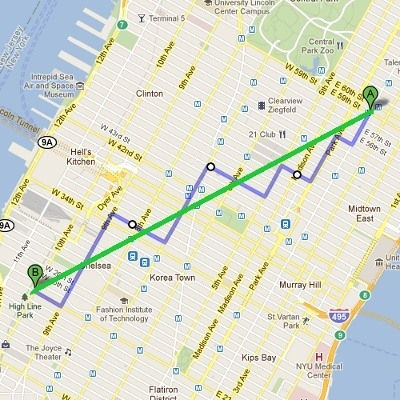
\includegraphics{MvsE}

\subsubsection{Cosine Similarity}
When documents are represented as term vectors, the sim- ilarity of two documents corresponds to the correlation be- tween the vectors. This is quantified as the cosine of the angle between vectors, that is, the so-called cosine similar- ity. Cosine similarity is one of the most popular similarity measure applied to text documents, such as in numerous in- formation retrieval applications [21] and clustering too [9].
Given two documents t a and t b, their cosine similarity is
\toadd{formule}
where t a and t b are m-dimensional vectors over the term set T = {t 1,\ldots, t m }. Each dimension represents a term with its weight in the document, which is non-negative. As a result, the cosine similarity is non-negative and bounded between [0,1].
An important property of the cosine similarity is its inde- pendence of document length. For example, combining two identical copies of a document d to get a new pseudo docu- ment d 0, the cosine similarity between d and d 0 is 1, which means that these two documents are regarded to be iden- tical. Meanwhile, given another document l, d and d 0 will have the same similarity value to l, that is, sim (t d, t l) = sim (t d 0, t l). In other words, documents with the same com- position but different totals will be treated identically. Strictly speaking, this does not satisfy the second condition of a met- ric, because after all the combination of two copies is a differ- ent object from the original document. However, in practice, when the term vectors are normalized to a unit length such as 1, and in this case the representation of d and d 0 is the same.
\includegraphics{CvsE}

\subsubsection{Jaccard Coefficient}
The Jaccard coefficient, which is sometimes referred to as the Tanimoto coefficient, measures similarity as the intersection
divided by the union of the objects. For text document, the Jaccard coefficient compares the sum weight of shared terms to the sum weight of terms that are present in either of the two document but are not the shared terms. The formal definition is:
\toadd{formule}
The Jaccard coefficient is a similarity measure and ranges between 0 and 1. It is 1 when the t a = t b and 0 when t a and t b are disjoint, where 1 means the two objects are the same and 0 means they are completely different. The corresponding distance measure is D J = 1 − SIM J and we will use D J instead in subsequent experiments.

\subsubsection{Pearson Correlation Coefficient}
Pearson’s correlation coefficient is another measure of the extent to which two vectors are related. There are different forms of the Pearson correlation coefficient formula. Given the term set T = {t 1,\ldots,t m }, a commonly used form is
\toadd{formule}
This is also a similarity measure. However, unlike the other measures, it ranges from +1 to −1 and it is 1 when t a = t b. In subsequent experiments we use the corresponding distance measure, which is D P = 1−SIM P when SIM P ≥ 0 and D P = |SIM P | when SIM P < 0.

\subsubsection{Averaged Kullback-Leibler Divergence}
In information theory based clustering, a document is con- sidered as a probability distribution of terms. The similarity of two documents is measured as the distance between the two corresponding probability distributions. The Kullback- Leibler divergence (KL divergence), also called the relative entropy, is a widely applied measure for evaluating the dif- ferences between two probability distributions.  
Given two distributions P and Q, the KL divergence from distribution P to distribution Q is defined as
\toadd{formule}
In the document scenario, the divergence between two dis-
tribution of words is:
\toadd{formule}
However, unlike the previous measures, the KL divergence is not symmetric, ie. D KL (P kQ) 6 = D KL (QkP). Therefore it is not a true metric. As a result, we use the averaged KL divergence instead, which is defined as
\toadd{formule}
The average weighting between two vectors ensures symme- try, that is, the divergence from document i to document j is the same as the divergence from document j to document i. The averaged KL divergence has recently been applied to clustering text documents, such as in the family of the Information Bottleneck clustering algorithms [18], to good effect.

\subsubsection{Kiti}
\begin{itemize}
	\item Manheteno
	\item Euklido
	\item Euklido atstumo kvadratas
	\item Čebyševo atstumas 
	\item Minkowski atstumas 
	\item Kosinuso atstumas 
	\item Žakardo atstumas 
	\item Daiso atstumas 
\end{itemize}

\subsection{Algoritmų rūšys}
\note{Kita skistymo versija}
Duomenų klasterizavimo algroritmai bendrai gali būti suskirstyti į\cite{kadhim2014text}: 
\begin{itemize}
	\item \ltang{\textbf{Padalijimo metodai}}{Partitioning methods}
	\item \ltang{\textbf{Herarkiniai metodai}}{Hierarchical methods}
	\item \ltang{\textbf{Tankumu paremti metodai}}{Density-based methods}
	\item \ltang{\textbf{Tinkliniai metodai}}{Grid-based methods}
	\item \ltang{\textbf{Modeliu paremti metodai}}{Model-based methods}
	\item \ltang{\textbf{Dažni struktūriniai metodai}}{Frequent pattern-based clustering}
	\item \ltang{\textbf{Suvaržymu paremti metodai}}{Constraint-based clustering}
	\item Papildomi, pritaikomi Web dokumentų klasterizacijai\cite{oikonomakou2005review} 
	\item \ltang{\textbf{Grafų metodai}}{Graph based clustering}
	\item \ltang{\textbf{Neuroninių tinklų metodai}}{Neural Network based clustering}
	\item \ltang{\textbf{Tikimybiniai metodai}}{Probabilistic clustering}
	\item \ltang{\textbf{Ontologiniai metodai}}{Ontological clustering}
	\item \ltang{\textbf{Nuorodomis paremti metodai}}{Link-based clustering}
\end{itemize}

Dar kiti suskirstymai rementis wikipedia
\begin{itemize}


    \item Jungiantys modeliai: pavyzdžiui, hierarchinė klasterizacija nubraižo modelį remiantis jungčių atstumais.
    \item Centroidiniai modeliai: pavyzdžiui, k-vidurkių algoritmai aprašo kiekvieną klasterį vienu vektorių vidurkiu.
    \item Pasiskirstymo modeliai: klasteriai modeliuojami remiantis statistiniais pasiskirstymais, pavyzdžiui kelių kintamųjų normalinis pasiskirstymas naudojamas lūkesčių-maksimizavimo algoritmo.
    \item Tankio modeliai: pavyzdžiui, DBSCAN ir OPTICS aprašo klasterius kaip tankius regionus duomenų erdvėje.
    \item Poerdvių modeliai: Biklasterizacija (taip žinoma kaip Ko-klasterizacija, ar dviejų-tipų-klasterizacija), klasteriai yra modeliuojami naudojant klasterių narius ir reikšmingas savybes.
    \item Grupiniai modeliai: kai kurie algoritmai nesuteikia išdirbto modelio gautiems rezultatams ir pateikia tik tam tikrą grupinę informaciją.
    \item Grafais-paremti modeliai: klika (tam tikra grupė su panašiais parametrais), kuri yra dalinis mazgų rinkinys grafe taip sujungtų, kad du mazgai tarpusavyje yra sujungti paviršiumi, kuris laikomas prototipine klasterio forma. Tam tikrų jungčių atpalaidavimas yra vadinamas kvazi-klikomis HCS klasterizacijos algoritmas.
\end{itemize}


Padalinjimo metodai sugeneruoja nepersidengenčių duomeų \ltang{pogrupius}{subset} taip, kad kiekvienas duomuo yra tik viename pogrupyje. Šiems metodams reikia išanksto nurodyti kiek klasterių norima turėti. Keletas šio tipo technikų: k-means ir variacijos of k-means-bisecting, k-medoids, PAM (Kaufman and Rousseeuw, 1987), CLARA (Kaufmann and Rousseeuw, 1990), CLARANS (Ng and Han, 1994)\ldots

Herarchiniai metodai sugenretuoja \ltang{}{nested} grupe klasterių kurie yra suskirstyti pagal medžio struktūrą. Šie algoritmai papildomai skirstomi į:\\
	\ltang{aglomeraciniai}{agglomerative} – dar kitaip žinomi kaip \ltang{iš apačios į viršų}{bottom-up} iš pradžių duomenis laiko kaip atskiras klasterio dalis ir nuosekliai jungia poras artimiausių klasterių į naujus tol kol visi klasteriai sujungiami į vieną.\\
	\ltang{diviziniai}{divisive} – dar kitaip žinomas kaip \ltang{iš viršaus į apačią}{top-down} iš pradžių visi duomenys priskiriami vienam klasteriu ir padalijimai yra atliekami rekursyviai besileidžian herarchija.Viešai prieinamos herarchinės technikos yra ROCK [4], Chamelon [5], BIRCH [6] and UPGMA.\needsource{išimk reikalingas citatas} \\
	Tankumo technikos sugrupuoja duomenis kurie yra pakankamai arti vieni kitų (tankūs), o retai išsidėsčiusius duomenis laiko \ltang{triukšmu}{noise} ir yra nepriskiremi jokiam klasteriui. Viešai prieinamos technikos yra DBSCAN ir praplėtimai, OPTICS and DENCLUE [6].\\
	Tinkliniai metodai naudoja \ltang{skirtingos raiškos}{multi\textendash{} resolution} tinklelio struktūrą duomenų surinkimui. Pagrindinis šios technikos privalumas \textendash{} našumas.\\
	Modelinės technikos gauna nurodumus kaip turi atrodyti klasteriai ir tada bando kiek galima geraiu joms pritaikyti duomenis.\\
	Dazniu paremti modeliai, as ju kolkas nesuprantu.\\
Suvaržymų (reikalavimų) paremti metodai naudojasi vartotojo ar programos nurodytais reikalavimais.\toadd{better explenation}

\subsection{Algoritmų skirstymas}
Klasteringo algoritmai skirstomi į šiuos tipus:
\begin{itemize}
	\item \textbf{monothetic }– visi populiacijos nariai turi kažkokia bendrą savybę (vyrai nuo 20 iki 25 metų amžiaus)
		\\\textbf{polythetic }– nariai yra panšūs, bet neturi konkrečios bendros savybės (kai atstumas tarp narių nurodo priklausomybę grupei)
	\item \ltang{\textbf{kieti}}{hard} klasteriai – kai grupės neturi bendrų elementų. Kartais gali susidaryti atvėjai kai elementas “matematiškai” priklauso ne vienai grupei. Nortin išlaikyti determiniškumą tokiu atveju reikia nurodyti pasirinkimo taisykle.
		\\\ltang{\textbf{minkšti}}{soft} klasteriai – kai grupės gali turėti bendrų elementų. Tokiu atveju galime nagrinėti kaip konkretus elementas priklauso skirtingoms grupėms ir kaip gerai jas atitinka.
	\item \ltang{\textbf{plokšti}}{flat} – kai elementai suskirstomi į grupes, kurios viena kitai yra lygios.
		\\\ltang{\textbf{herarkiški}}{hierarchical} (taxonomy) – Kai grupė gali būti sudaryta iš kelių “konkretesnių” grupių. Pvz.\ retryveris $\,\to\,$ šuo $\,\to\,$ žinduolis $\,\to\,$ gyvūnas
\end{itemize}
Šiame skyriuje apžvelksiu algoritmų:

\iffalse{}
\begin{table}[H]\footnotesize
  \centering
  \caption{Lentelės pavyzdys}    % Antraštė įterpiama prieš lentelę
  {\begin{tabular}{lccc} 
	\toprule
	Algoritmas & \multicolumn{3}{c}{Tipas} \\
	\midrule
	%K-mean & hard & flat & polythetic \\ %\midrule
	%Hierarchical & hard & x & x\\
	\bottomrule
  \end{tabular}}
\end{table}
\fi{}

\subsubsection{K-means}
\ltang{K-vidurkių}{K-mean} algoritmas suskirsto duomenis į nurodytą ($ k $) klasterių. \[ \underset{\mathbf{S}} {\operatorname{\arg \min}}  \sum_{i=1}^{k} \sum_{\mathbf x \in S_i} \left\| \mathbf x - \boldsymbol\mu_i \right\|^2 \]
Praktikoje dažniausiai naudojamas duodama $n$ vektroių (su $d$ dimensijų) ir numeris $k$.  Sustatome $k$ centroidų $c$ į atsitiktines vietas.
\begin{enumerate}
	\item Kiekvienam taskui (vektoriui) randame artimiausia c
	\item Kiekviena centroida pakeiti taip kad jis geriau atitiktu jam priskirtą klusterį (sumažinti atstuma iki visų taškų arba kitaip tariant rasti taškų centrą). Tada eini i žingsni  1.\ %TODO add proper reference
	tol kol visi klusteriai išlieka vienodi.
\end{enumerate}
\BigO{iteracijos*K*n*d} produce hard, flat, polythetic cluster. 

%\subsection{mixture models}
\subsubsection{Hierarchinis klasterizavimas}
\ltang{Hierarchical}{Hierarchinis} klasterizavimo algoritmai yra viena iš populiariausių dokumentų klasterizavimo algoritmų grupė. Hierarchinis klasterizavimo algoritmas plačiai naudojamas iki šių dienų, nors šis algoritmas yra vienas iš pirmujų klasterizavimo algoritmų. Šis algoritmas labiausiai tinkamas naudoti klasterizuojant nedidelius duomenų rinkinius. Pradžioje hierarchinis algoritmas nustato bendrą visų klasterių tarpusavio priklausomybių struktūrą, ir tik tada sprendžia koks klasterių skaičius yra optimalus [11]. Hierarchinio klasterizavimo sudėtingumas: \BigO{n^3}.\\
Hierarchinis klasterizavimo algoritmas skirstomas į du algoritmus: jungimo ir skaidymo.
\begin{itemize}
	\item \ltang{Skaidymo}{divisive} algoritmas – pradinis klasteris susideda iš visos duomenų aibės ir nuosekliai dalinamas į smulkesnius klasterius.
	\item \ltang{Jungimo}{agglomerative} algoritmas – pradinis klasteris susideda iš vieno objekto ir prie jo jungiant kitus objektus (duomenis) gaunami vis didesni klasteriai, kol gaunamas vienas didelis klasteris.
\end{itemize}
\includegraphics{hierargram}
Hierarchinio klasterizavimo algoritmo atstumai tarp klasterių skaičiuojami keliais metodais:
\begin{itemize}
	\item \ltang{Artimiausias atstumas}{Single-link},
	\item \ltang{Tolimiausias atstumas}{Complete-link},
	\item Vidutinis atstumas,
	\item Centroidės atstumas,
	\item Ward atstumas – Euklido atstumo sumos kvadrato minimumas.
\end{itemize}
Šiuo metu populiariausiais laikomi 1 Artimiausio atstumo ir 2 Tolimiausio atstumo algoritmai.  Single-link algoritmas kuris dar žinomas kaip mažiausias skaičiuoja dviejų objektų atstumą kuris yra prilyginamas atstumui tarp dviejų artimiausių objektų. Complete-link algoritmas kuris žinomas kaip didžiausias skaičiuoja dviejų objektų atstumą, kuris yra prilyginamas atstumui tarp dviejų tolimiausių objektų.

\subsubsection{EM}
\ltang{EM}{Expectation maximization} algoritmas kitaip dar vadinamas tikimybinis klasterizavimo algoritmas.  Tegul stebinys $X$ priklauso vienai iš $q$ skirtingų klasių, kur $v$ žymi stebimos klasės numerį $f_i(x)$ – sąlyginis pasiskirstymo tankis kai $v = i$. Klasterizuojant tokią imtį daroma prielaida, kad $f_1,f_2,\ldots,f_q$ yra normaliniai pasiskirstymo tankiai su vidurkiais $M(i)$ ir kovariacinėmis matricomis $R(i)$.\\
\begin{equation}
	f(x)=\sum^q_{i=1} {q_i f_i (x) = f(x, \theta)}
\end{equation} 
Tada
Kur $\theta$ yra visų parametrų vektorius.\\
Klasterizavimas remiasi aposteriorinių tikimybių
\begin{equation}
	\pi_i (x) = P\{v = i |X = x\} = \frac{p_i f_i(x)}{f(x,\theta)}
\end{equation} 
vertinimu\\
$v(X) = argmaxi \pi_i(X)$\\
EM algoritmas yra rekurentinė procedūra, skirta $\theta$ maksimalaus tikėtinumo įverčio ir jį atitinkančių $\pi_i$ įverčių apskaičiavimui.
\includegraphics{temp0}
Taigi, pasiskirstymo tankio funkcija $f(x)$ statistinį vertinimą, kai imtis yra klasterizuojama į $q$ klasterių $X = \{X(1), X(2), \ldots, X(n)\}$ siūloma atlikti dviem etapais:\\
Griežto klasterizavimo – kai $X = K_1\cup  \ldots \cup K_q$, kur kiekvienas $X(t)$ priklauso vienam ir tik vienam klasteriui $K_i$, kai $i = 1, 2, \ldots, q$.
Negriežto klasterizavimo – kai klasteriai $K_i$ suprantami kaip aibės $\{(X(1), \pi_i (1)), \ldots, (X(n), \pi_i(n))\}$, kur $\pi_i(t)$ rodo su kokiu svoriu (tikimybe) stebinys $X(t)$ priskiriamas klasei $K_i$. Mišinio komponentai $f_i(x)$ vertinami pagal klasterio $K_i$ elementus, taikant vieną iš žinomų neparametrinio vertinimo metodų.
\includegraphics{EM}

\subsubsection{Tolimiausio kaimyno}
\ltang{Tolimiausio kaimyno}{Farthest First}klasterizavimo algoritmas, kuris visus duomenis skisto į klasterius palaipsniui – sukuria po vieną naują klasterį kiekvienoje iteracijoje. Pirmuoju žingsniu visi duomenys priskiriami vienam klasteriui, tame klasteryje surandami du duomenys kurie labiausiai skiriasi vienas nuo kito. Tuomet, pradinis klasteris išskaidomas į du naujus klasterius, kurių pradiniai duomenys skaidomojo klasterio labiausiai besiskiriantys duomenys. Kol nepriskirti kiti duomenys, tol jie sutampa su išskaidytų klasterių centroidais. Paskui likę duomenys priskiriami vienam iš naujai sukurtų dviejų klasterių. Pirmoje iteracijoje pasirenkamas vienas klasteris, pagal tam tikrus kriterijus ir jis vėl skaidomas į du naujus klasterius. Kriterijai gali būti įvairūs – klasterio dydis, maksimalus klasterio diametras, ir pns. Klasterių skaidymas vykdomas tol, kol gaunamas reikiamas kiekis klasterių.\\
\includegraphics{FF}

\subsubsection{DBSC}
\toadd{Koks skirtumas lyginant su DBSCAN}
\ltang{DBSC}{Density Based Spatial Clustering} tai duomenų tankiu pagrįstas klasterizavimo metodas, kaimyninius duomenis grupuojantis į klasterius ne pagal atstumo matą, o pagal objektų tankį. Tankis tai minimalus taškų atstumas, tarp kurių yra tam tikras atstumas. Taškai, kurie nutolę tam tikru nustatytu atstumu vienas nuo kito, vadinami kaimynais. Pagal tam tikrą tankio funkciją arba pagal kaimynystės tankį yra sudaromi klasteriai. Sudėtingos struktūros klasterius sugeba atskirti tankiu grindžiami algoritmai. Šie algoritmai taškų atsiskyrėlių neįtraukia į klasterius.
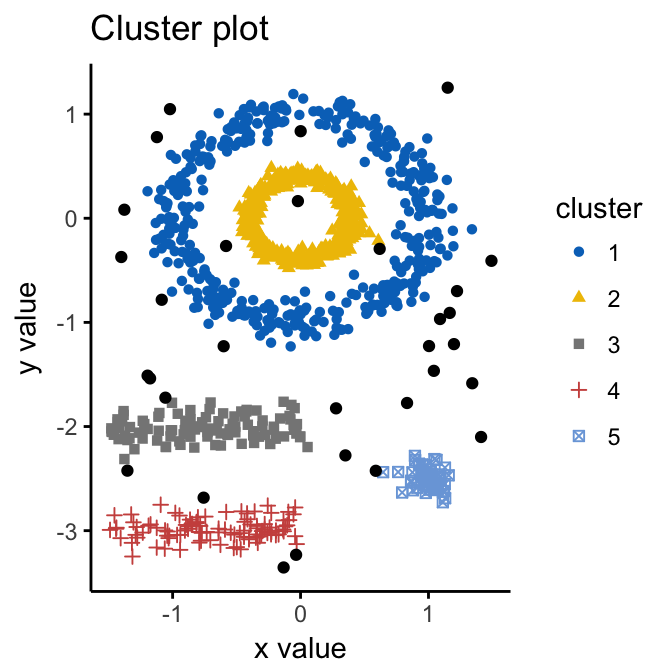
\includegraphics{DBSCAN}

\subsubsection{Fuzzy k-means}
Fuzzy k-means klasterizavimas yra vienas iš populiariausių klasterizavimo algoritmų k-means išplėtimas. K-means klasterizavimas suskirsto duomenis į atskiras grupes, kai vienas objektas gali priklausyti tik vienam klasteriui, tuo tarpu fuzzy k-means klasterizavimo algoritmas duomenis suskirsto į klasterius, kai objektas gali priklausyti skirtingoms grupėms (klasteriams) su tam tikra tikimybe.\\
Fuzzy k-means klasterizavimo algoritmo veikimas yra toks: kiekvieno aibės objekto priklausomybė bet kokiam klasteriui $k$ yra neapibrėžta. Aibės objektai klasteriams priklauso su tikimybėmis $P(wi | xj, \theta)$, kur $\theta$ – duomenų vektorius priklausomybių funkcijoms. Fuzzy k-means klasterizavimo algoritmas stengiasi sumažinti kainų funkciją Jfuz:
\begin{equation}
	Jfuz=\sum{(\sum{(P(wi|xj,\theta)b‖xj−μi‖2)}nj=1)}ci = 1,
\end{equation}
kur kintamasis $b$ reguliuoja skirtingų klasterių persidengimą.\\
Visoms duomenų aibėms klasteriai turi sureguliuoti svorius, atsižvelgiant į pateiktų duomenų atstumus, bei klasterių svorius, kurie nusako tikimybes ar duomenų aibės priklauso pateiktiems klasteriams. Fuzzy k-means klasterizavimo sudėtingumas:\BigO{ndc^2i}.
\includegraphics{FKM}

\subsubsection{Dirichlet}
Dirichlet klasterizavimas yra $p$ vektorių tikimybių pasiskirstymo funkcija. Visi vektoriai $p$ atspindi duomenų pasiskirstymo tikimybes $a$. Dirichlet klasterizavimas apibrėžiamas vektoriumi $ \alpha = {\alpha i}i=1|A+|$, kai $ \alpha i > 0$,\\
\begin{equation}
	(p|\alpha)=\Gamma(|\alpha|)\Pi i=1|A|\Gamma (\alpha i)\Pi i=1|A|pi \alpha i−1,
\end{equation}
čia $\Pi$ (.) žymi – gama funkciją, $\sum{pi=1|A|i=1}$, bei $|\alpha| = \sum{\alpha i|A|i=1,pi≥0} (i =1,\ldots,|A|)$.
Dirichlet klasterizavimas paremtas individualių klasterių matematine kombinacija, kuri naujai sukuria tikimybių pasiskirstymą. Visiems skirtingiems klasteriams suteikiami svoriai, jie vadinami koeficientais. Klasterių paskirstymas $\varphi$, kuris sudarytas iš $l$ komponentų, gaunamas iš:
\begin{equation}
	\varphi = \sum{qjgjlj=1},
\end{equation}
$gj$ – yra Dirichlet klasteriai. Kiekvienas klasteris aprašo pasiskirstymo dėsnį. Duomenų skaičius klasteriuose yra neribojamas, tačiau naudojant didelį kiekį duomenų šis metodas veikia neoptimaliai.

\subsubsection{Affinity Propagation}
\subsubsection{Mean Shift}
\subsubsection{Spectral clustering}
\subsubsection{Birch}


\subsubsection{Binarization of consensus partition matrices}
\subsubsection{Canopy clustering algorithm}
\subsubsection{Cluster-weighted modeling}
\subsubsection{Cobweb}
\subsubsection{Complete-linkage clustering}
\subsubsection{Constrained clustering}
\subsubsection{CURE data clustering algorithm}
\subsubsection{Data stream clustering}
\subsubsection{DBSCAN}
\subsubsection{FLAME clustering}
\subsubsection{Fuzzy clustering}
\subsubsection{Hoshen–Kopelman algorithm}

\subsection{Kiti metodai}

\subsection{Latent Dirichlet allocation}
Latent Dirichlet allocation (toliau LDA, nesumaišyti su Linear discriminant analysis, kas yra kitas mašininio mokymosi metodas). Yra kurkas sudetingesnis dokumentu analizavimo metodas. Kartais priskiremas atskirai algoritmu klasei Topic modeling, kuri bando ne grupuoti duomenis o suteigti jiems temas. Palyginant su praeitais metodais dokumentai turėjo priklausyti vienai iš klasterių ar jų herarkijai, bet dokumentas gali turėti kelias temas. 
% Reikia perkelti ir tiksliau apibrėžti ką būtent gražina.	
Todėl LDA gražina ne sugrupuotus duomenis, o pasiskirstymą kiek kokių temų turi kiekvienas dokumentas  

\section{Algoritmų testavimas/Kokybės vertinimas}
\toadd{purity and entropy}
Viena iš fundamentalių neprižiūrimo mokymosi problemų yra modelių testavimas. Skirtingai nei „prižurimame mokymasi“ kur svarbu atdidėti dali duomenų su kuriais nėra mokomasi o tik testuojama sugeneruoti modeliai, „neprižiurimame mokymasi“ mes to nelgalim atlikti\ldots Bet egzsituoja keltatas metodu kaip galima patikrinti sudarytus klasterius.
\begin{itemize}
	\item Pirma galima sugeneruotus klasterius leisti tikrinti \textbf{žmonėms }. Tam yra keli būdai. Galima tiesiog duoti sugeneruotus klasterius ir bandyti nuspresti ar jie tinkami. Taipat galima parainkti du atsitiktinius dokumentus ir spėti ar jie turėtu būti viename ar atskiruose klasteriuose, ir tada palyginti su kompiuterio sugeneruotu rezultatu. 
	\item Taip yra metodų kaip atlikti testavimą automatiškai. Vienas jų paimti 2(ar daugiau) dokumentus iš skirtingų klasterių ir apkeisti juos vietomis, tada patikrinti klasteriu //stipruma. Tai atlike dokybe kartų galime spręsti kaip sėkmingai sekėsi klasterizacija, jeigu apmainant jų kokybė nukrito tai reikškia, kad dokumentai sėkmingai suklaserizuoti, bet jeigu nesikeite tai reiške, kad klasteriai mažai vienas nuo kito skiresi ir klasreizacija nesekminga.
\end{itemize}

\section{Rezultatų vizuoalizacija}
Dažnai norėdami geriau pažinti (ar testuoti) klasterizacijos rezultatus mes galime juo vizuolizuoti. Vizulaizacijos gali buti įvairios ir dažnai priklauso nuo algoritmo rūšies, bet dažniausiai naudojama \textbf{point cloud} vizualizacijos. Jose matosi pagal kokius parameturs (ašis) buvo klasterizuojama ir kaip atrodo sudaryti klasteriai.Taip pat galima pridėti papildomų indikatorių, priklausomų nuo algoritmo. Pavyzdžiui klasteriams sudarytiems k-means metodu galima nubraižyti atitinkamus „centrinius taškusn“.

\section{Susijusios, aktuoalios problemos}
\subsection{Keyword extraction}
\subsection{Cluster labeling}
\subsection{Document Classification}
\subsection{Dimensionality reduction}
Dimensionality reduction methods can be considered a subtype of soft clustering; for documents, these include latent semantic indexing (truncated singular value decomposition on term histograms) and topic models.
\sectionnonum{Išvados}
%Išvadose ir pasiūlymuose, nekartojant atskirų dalių apibendrinimų, suformuluojamos svarbiausios darbo išvados, rekomendacijos bei pasiūlymai.


\printbibliography[heading=bibintoc] % Literatūros šaltiniai aprašomi
% bibliografija.bib faile. Šaltinių sąraše nurodoma panaudota literatūra,
% kitokie šaltiniai. Abėcėlės tvarka išdėstoma tik darbe panaudotų (cituotų,
% perfrazuotų ar bent paminėtų) mokslo leidinių, kitokių publikacijų
% bibliografiniai aprašai (šiuo punktu pasirūpina LaTeX). Aprašai pateikiami
% netransliteruoti.

\appendix  % Priedai
% Prieduose gali būti pateikiama pagalbinė, ypač darbo autoriaus savarankiškai
% parengta, medžiaga. Savarankiški priedai gali būti pateikiami kompiuterio
% diskelyje ar kompaktiniame diske. Priedai taip pat vadinami ir numeruojami.
% Tekstas su priedais siejamas nuorodomis (pvz.: \ref{img:mlp}).

\end{document}
